\documentclass{article}
\usepackage{iclr2025_conference}
\usepackage{amsmath,amssymb}
\usepackage{graphicx}
\usepackage{booktabs}
\usepackage{xcolor}
\usepackage{natbib}
\usepackage[colorlinks=true,allcolors=blue]{hyperref}
\graphicspath{{figures/}}

\newcommand{\PKPS}{PKPS\xspace}
\usepackage{xspace}

\title{Product Kernel Perspective Spaces:\\ Predicting Benchmark Scores from Sparse, Unpaired Model Evaluations}
\author{Anonymous}

\begin{document}
\maketitle

\begin{abstract}
Evaluating language models is expensive, and in practice benchmark coverage is
sparse: many models, many tasks, but each model is run on only a subset of tasks,
and within a task on only a subset of queries. The Data Kernel Perspective Space
(DKPS) embeds models from their responses and predicts held-out scores, but it
requires a \emph{paired} design---every model must answer the same queries---so it
discards the abundant unpaired evaluations real benchmarks produce. We introduce
the \textbf{Product Kernel Perspective Space (\PKPS)}, which replaces DKPS's
implicit identity matching of queries with a \emph{product kernel}
$k_Q \cdot k_R$ that weights response comparisons by query similarity. \PKPS
recovers DKPS exactly in the paired limit (as the query-kernel bandwidth
$\sigma\!\to\!0$) and degrades gracefully when models answer different queries. On
synthetic data we map how prediction accuracy depends on the number of models,
task sparsity, query sparsity, and task structure. On the HELM benchmark we study
two regimes with their domain-standard baselines: (i) \emph{missing queries}
(efficient benchmarking), where \PKPS matches item-response theory (IRT) when data
is paired but, unlike IRT and DKPS, does not collapse as queries unpair; and (ii)
\emph{missing tasks} (benchmark completion), where \PKPS is competitive with
low-rank matrix completion and wins decisively when few models are available. We
then scale to a single heterogeneous suite of $18$ tasks and $93$ models spanning
math, translation, medical QA, and legal classification, using a block-diagonal
product kernel that places rich-text and single-token responses in one space: \PKPS
roughly halves the error of naive sampling for efficient evaluation across the
suite. In every regime an ensemble of \PKPS with the domain baseline is the most
robust predictor, indicating the embedding and score-only signals are complementary.
\end{abstract}

\section{Introduction}
Comprehensive evaluation of language models is a growing bottleneck: leaderboards
track hundreds of models across dozens of benchmarks, yet no model is run on
everything. The resulting (model $\times$ task) score matrix is \emph{doubly
sparse}. \emph{Across tasks}, a model is evaluated on a subset of benchmarks
(missing tasks). \emph{Within a task}, evaluation may use only a subset of queries
to save cost (missing queries). Predicting the missing entries---a model's score on
a task it has not been (fully) run on---would let practitioners reuse cached
evaluations instead of paying to re-run them \citep{polo2024tinybenchmarks,
vivek2024anchor, benchpress}.

The Data Kernel Perspective Space (DKPS) \citep{dkps_qeff} is a black-box approach:
it embeds each model from its query responses, places models in a low-dimensional
Euclidean space via classical multidimensional scaling, and regresses benchmark
scores in that space. DKPS is query-efficient and competitive with item-response
theory. But it has a structural limitation: the distance between two models is the
average squared difference of their responses \emph{to the same queries}, so DKPS
requires a \emph{paired} design. When models answer different queries---the common
case in real, organically-assembled leaderboards---DKPS has nothing to compare and
the information in those unpaired responses is thrown away.

We introduce the \textbf{Product Kernel Perspective Space (\PKPS)}. The key change
is to compare responses to \emph{similar} queries, not only identical ones, by
weighting each response-pair comparison with a query kernel. This (i) lets every
unpaired response contribute, and (ii) contains DKPS as the special case where the
query kernel is the identity. Our contributions:
\begin{itemize}
\item \textbf{Method.} A product-kernel distance $k_Q\cdot k_R$ that generalizes
DKPS, reduces to it as the query-kernel bandwidth $\sigma\!\to\!0$, and whose
bandwidth is chosen per run by a cheap median-scaled cross-validation
(Section~\ref{sec:method}).
\item \textbf{Synthetic study} of how accuracy scales with the number of models,
task sparsity, query sparsity, and task spread (Section~\ref{sec:synthetic}).
\item \textbf{Missing queries (RD1).} Using HELM-MATH as a running example, \PKPS
recovers the query-efficiency of DKPS in the paired regime and---unlike DKPS and
IRT, which both collapse---remains accurate as queries unpair (Section~\ref{sec:rd1}).
\item \textbf{Missing tasks (RD2).} \PKPS is competitive with low-rank matrix
completion, wins when models are scarce, and an ensemble of the two is best, showing
the embedding and low-rank signals are complementary (Section~\ref{sec:rd2}).
\item \textbf{Joint heterogeneous suite.} Our main result evaluates both regimes on
a single $18$-task, $93$-model benchmark spanning math reasoning, translation,
medical QA, and legal classification (Section~\ref{sec:joint}). A block-diagonal
product kernel handles datasets with rich text responses and with single-token
answers in one space. \PKPS roughly halves the cost of efficient evaluation across
the suite; for benchmark completion the suite matrix is low-rank and matrix
completion is strong, but the \PKPS ensemble remains the most robust predictor.
\end{itemize}

\section{Background and method}
\label{sec:method}

\paragraph{Paired DKPS.} Let $x_{ij}=\mathrm{embed}(\mathrm{model}_i(q_j))$ be the
embedding of model $i$'s response to query $j$. With all $n$ models answering the
same $m$ queries, the DKPS squared distance is
$D^2(i,k)=\tfrac{1}{m}\sum_j \|x_{ij}-x_{kj}\|^2 = A_{ii}+A_{kk}-2A_{ik}$, where
$A_{ab}=\tfrac{1}{m}\sum_j k_R(x_{aj},x_{bj})$ and $k_R$ is a linear response
kernel. Classical MDS on $D$ yields model coordinates; a regressor maps coordinates
to benchmark scores. The sum over $j$ pairs response $j$ of model $a$ with response
$j$ of model $b$: an \emph{identity} matching of queries.

\paragraph{Product kernel.} \PKPS replaces identity matching with a query kernel
$k_Q$:
\begin{equation}
A_{ab} = \frac{\sum_{j\in Q_a}\sum_{l\in Q_b} k_Q(q_j,q_l)\, k_R(x_{aj},x_{bl})}
              {\sum_{j\in Q_a}\sum_{l\in Q_b} k_Q(q_j,q_l)},
\label{eq:A}
\end{equation}
where $Q_a$ is the set of queries answered by model $a$ and $q_j$ is the embedding
of query $j$. Each term is normalized by its own query-kernel mass, so models that
answered different numbers of (or entirely different) queries are still comparable.
Two limits are important:
\begin{itemize}
\item \textbf{$k_Q=\delta$ (identity)}: only $j=l$ survives, recovering paired DKPS.
\item \textbf{$k_Q$ RBF}: $k_Q(q_j,q_l)=\exp(-\|q_j-q_l\|^2/2\sigma^2)$ lets
responses to \emph{similar} queries---even across tasks---contribute, so unpaired
data is used.
\end{itemize}
As $\sigma\!\to\!0$ the RBF kernel converges to $\delta$ (distinct queries have
distinct embeddings), so \PKPS is a strict generalization of DKPS with DKPS as its
$\sigma\!\to\!0$ limit.

\paragraph{Choosing the bandwidth.} The optimal $\sigma$ depends on how paired the
data is: small when query overlap is high (recover exact matching), large when
overlap is low (bridge across queries). We set it per run by cross-validation over a
median-scaled grid $\sigma\in\{0.02,\dots,5\}\cdot\mathrm{med}$, where $\mathrm{med}$
is the median pairwise query distance. The selection signal differs by regime, and
this dictates how aggressively we tune. In the \emph{missing-queries} setting the
reference models' full scores are known and dense, so leave-one-family-out gives a
low-noise criterion and the grid search is reliable. In the \emph{missing-tasks}
setting only a sparse set of held-out cells is available; there we find held-out MAE
is flat in $\sigma$ for $\sigma\!\ge\!0.5\,\mathrm{med}$, so a fixed median bandwidth
is both simpler and more robust than per-run selection on the noisy split. One
response-kernel pass produces the entire $\sigma$-grid, so tuning is nearly free. We
use a single regressor (distance-weighted $k$-NN) and a logit-space, bias-decomposed
head throughout; the one quantity we always fit per run is the ensemble weight that
blends \PKPS with the domain baseline.

\paragraph{Estimation pipeline.} For each replicate we (i) reduce response and
query embeddings by PCA on the \emph{observed} rows only (dimension chosen by the
second Zhu--Ghodsi elbow); (ii) form $D$ from Eq.~\ref{eq:A}; (iii) embed models by
classical MDS; (iv) predict scores with a bias-decomposed, logit-space head---a
two-way (model $+$ task) additive model plus a regression of the residual on the
embedding---matching the normalization used by strong score-only baselines.

\section{Synthetic experiments}
\label{sec:synthetic}
We generate models with latent ability vectors $v_i$ and tasks with latent vectors
$t_k$, scores $v_i\cdot t_k+\epsilon$, and queries drawn near each task center.
Two-level missingness (task-level and query-level) mirrors real benchmarks.
Figure~\ref{fig:synthetic} sweeps, one at a time, the number of models, number of
tasks, task observation probability, query observation probability, task spread,
and response noise. The \emph{combined} estimator (all queries) consistently beats
the \emph{paired} (shared-task only) and \emph{unpaired} (unique-task only)
estimators, with the largest margin in the realistic regime: many models, sparse
task overlap, moderate task spread. The advantage shrinks when overlap is abundant
(paired already has the data it needs) or tasks are very dissimilar (the query
kernel cannot bridge them).

\begin{figure}[t]
\centering

\includegraphics[width=\textwidth]{fig_synthetic.pdf}
\caption{Synthetic study (held-out score MAE, 50 seeds). The combined product
kernel dominates the paired/unpaired estimators across the number of models, number
of tasks, task observation probability, query observation probability, task spread,
and response noise $\times$ queries-per-task.}
\label{fig:synthetic}
\end{figure}

\section{Missing queries: efficient benchmarking}
\label{sec:rd1}
Here each model is run on a few queries of a single benchmark and we predict its
\emph{full} benchmark score, leave-one-model-family-out. Baselines: the
\emph{sample} mean of answered queries; \emph{IRT} (1-PL Rasch), which fits item
difficulties on the largest fully-paired $|F|\times|Q|$ block of the observed
responses and predicts ability from the answered anchor items; and \emph{DKPS}
(identity query kernel). We report \PKPS with the adaptive bandwidth and an ensemble
of \PKPS with the sample mean (mixing weight fit per run). All use Gemini response
embeddings on 95 models / 39 families.

Figure~\ref{fig:rd1} shows three regimes. \textbf{(a) Query efficiency} (all models
answer the same $m$ queries): at a budget of one query, DKPS/\PKPS reach $0.14$ MAE
versus $0.35$ for the sample mean and $0.34$ for IRT; the sample mean catches up
only as the budget grows. \textbf{(b) The pairing cliff} (fix the budget at 16
queries, slide from fully paired to fully unpaired): IRT and DKPS are strong when
paired ($0.077$, $0.087$) but \emph{collapse} as queries unpair ($0.28$, $0.24$),
because neither has a dense block or shared queries to use; \PKPS degrades only
mildly ($0.09\!\to\!0.14$). \textbf{(c) Number of models}: both perspective methods
need a cohort to regress against and degrade together when models are scarce
($\sim\!0.19$ at $n{=}10$), converging as the cohort grows. The ensemble is best in
every panel: when the structured methods fail, it falls back to the sample mean; when
queries are few, it leans on the embedding.

\begin{figure}[t]
\centering
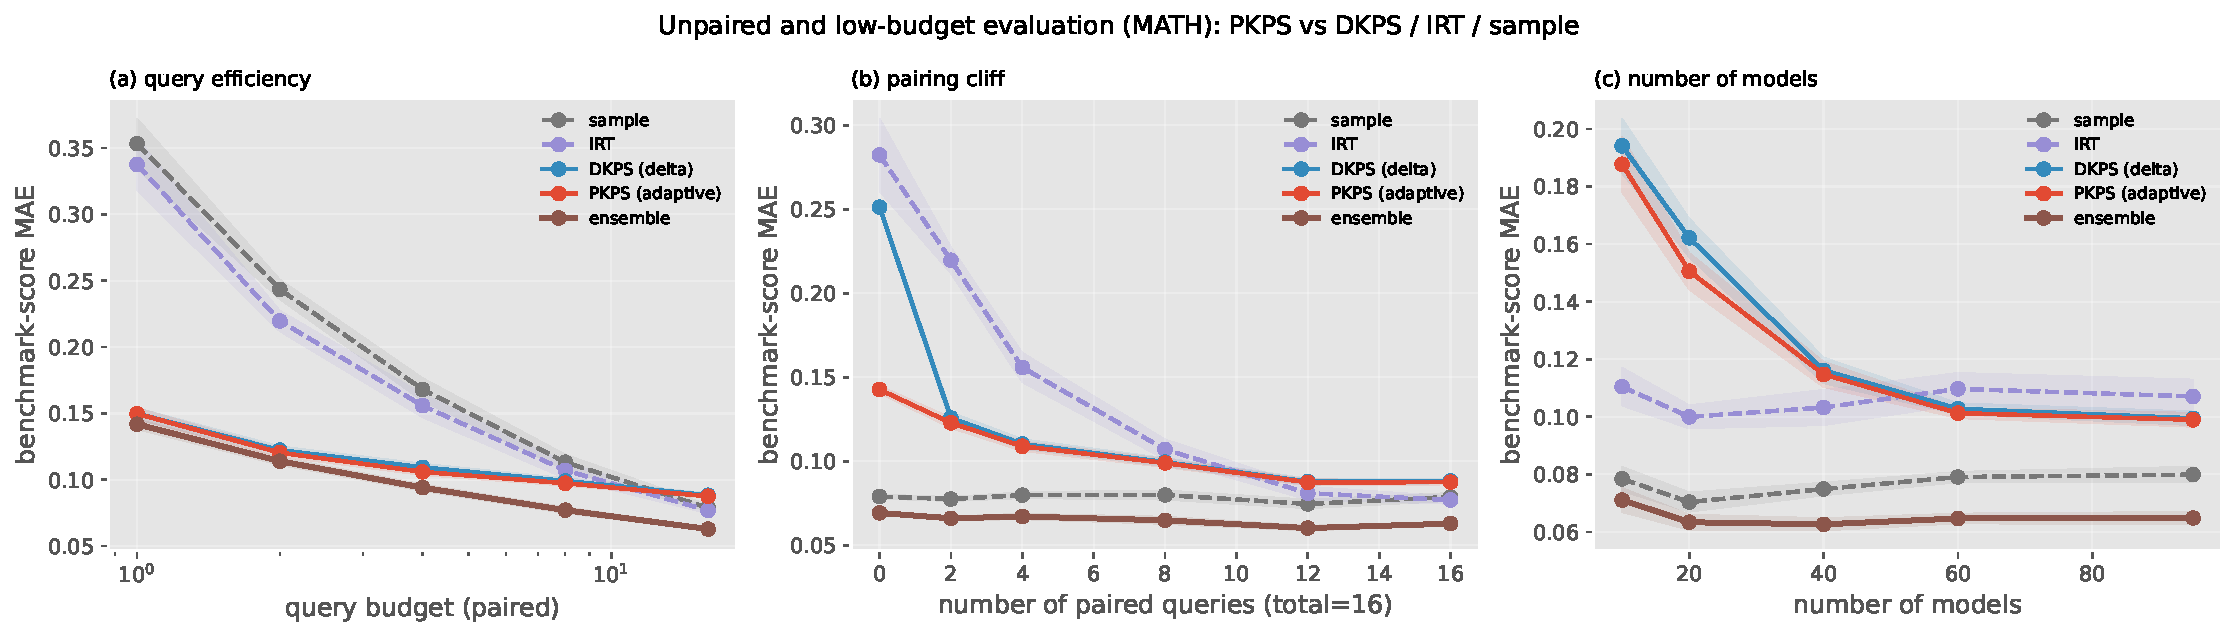
\includegraphics[width=\textwidth]{fig_rd1.pdf}
\caption{Missing queries on HELM-MATH (benchmark-score MAE, 20 seeds). (a) Query
efficiency: DKPS/\PKPS beat sample and IRT at low budget. (b) Pairing cliff: IRT and
DKPS collapse as queries unpair; \PKPS survives. (c) Number of models: DKPS collapses
with few models, \PKPS is robust. The ensemble is best throughout.}
\label{fig:rd1}
\end{figure}

The takeaway: in the \emph{paired} regime \PKPS reproduces the query-efficiency of
DKPS and IRT, but only \PKPS retains accuracy once evaluations are \emph{unpaired}
or models are scarce---the regimes that dominate real, organically-collected
leaderboards.

\section{Missing tasks: benchmark completion}
\label{sec:rd2}
Now we predict held-out (model, task) entries of a (model $\times$ task) matrix. The
domain-standard baseline is low-rank matrix completion: model-and-task biases plus a
rank-2 factor fit by alternating least squares in logit space \citep{benchpress}.
We compare \PKPS and an ensemble of the two, with the blend weight fit per run by
repeated held-out cross-validation. Each observed pair contributes its responses to
the embedding and its (sample) score to the completion; held-out MAE is measured
against the true full score.

\begin{figure}[t]
\centering
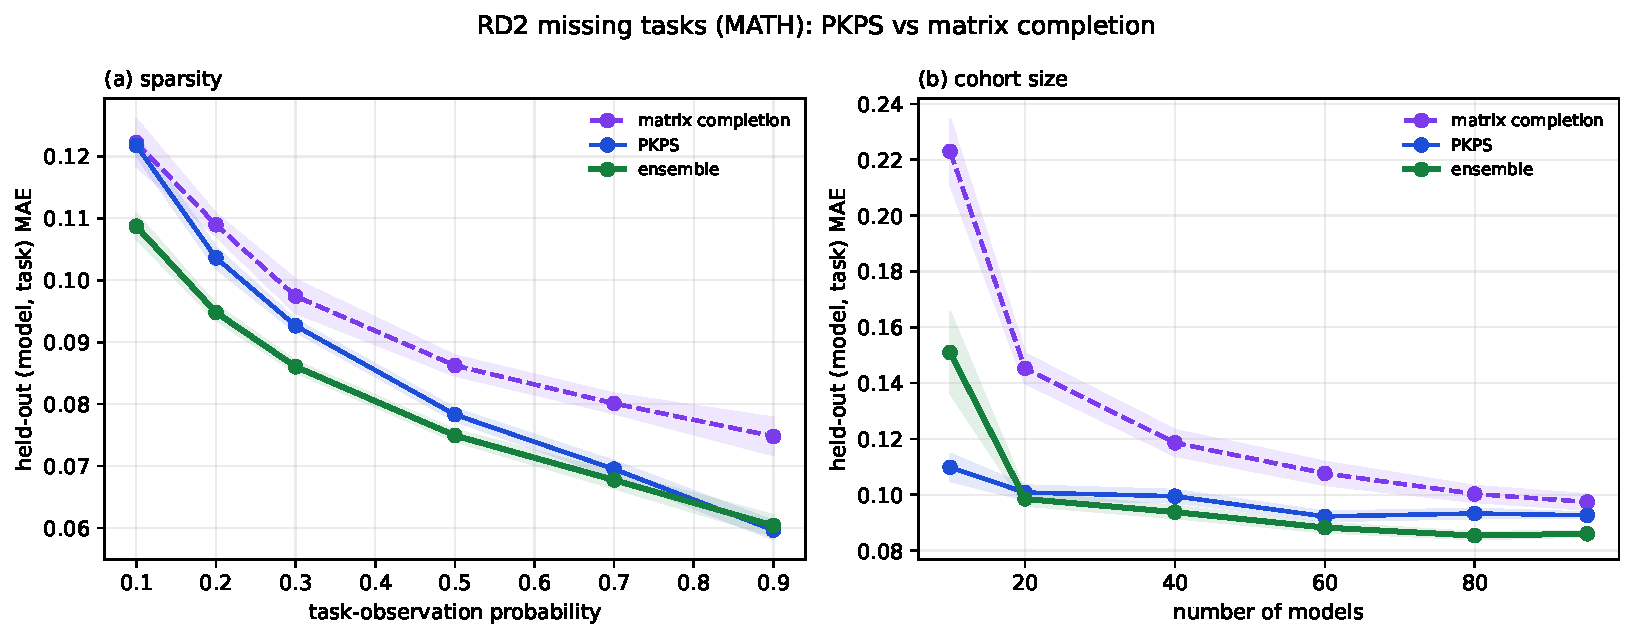
\includegraphics[width=\textwidth]{fig_rd2_main.pdf}
\caption{Missing tasks on HELM-MATH (held-out MAE). \PKPS beats matrix completion at
every task-observation probability (left); at every model count (right) matrix
completion collapses when models are scarce---rank-2 completion needs many rows---
while \PKPS stays flat ($2\times$ lower at $n{=}10$). The ensemble (green) is best
throughout, falling back to whichever component is stronger when the cohort is too
small to fit the blend.}
\label{fig:rd2main}
\end{figure}

On MATH (Figure~\ref{fig:rd2main}), \PKPS beats matrix completion at every
task-observation probability, and as the number of models shrinks matrix completion
collapses (rank-2 completion needs many rows) while \PKPS is flat---$2\times$ lower
at $n{=}10$. An \emph{ensemble} of the two is best at essentially every operating
point: the embedding and low-rank signals are complementary, and the cross-validated
weight defaults to the stronger component when the cohort is too small to fit a
blend. On WMT-14, whose continuous translation scores form a near-rank-one matrix,
the picture inverts: matrix completion is the stronger method and \PKPS trails, but
the ensemble stays competitive---the two datasets bracket the spectrum of matrix
rank. A per-task / per-model error breakdown (Figure~\ref{fig:rd2breakdown}) shows
the ensemble has the lowest error on all seven MATH subjects and shifts the entire
per-model error distribution down, rather than helping a few outliers.

\begin{figure}[t]
\centering
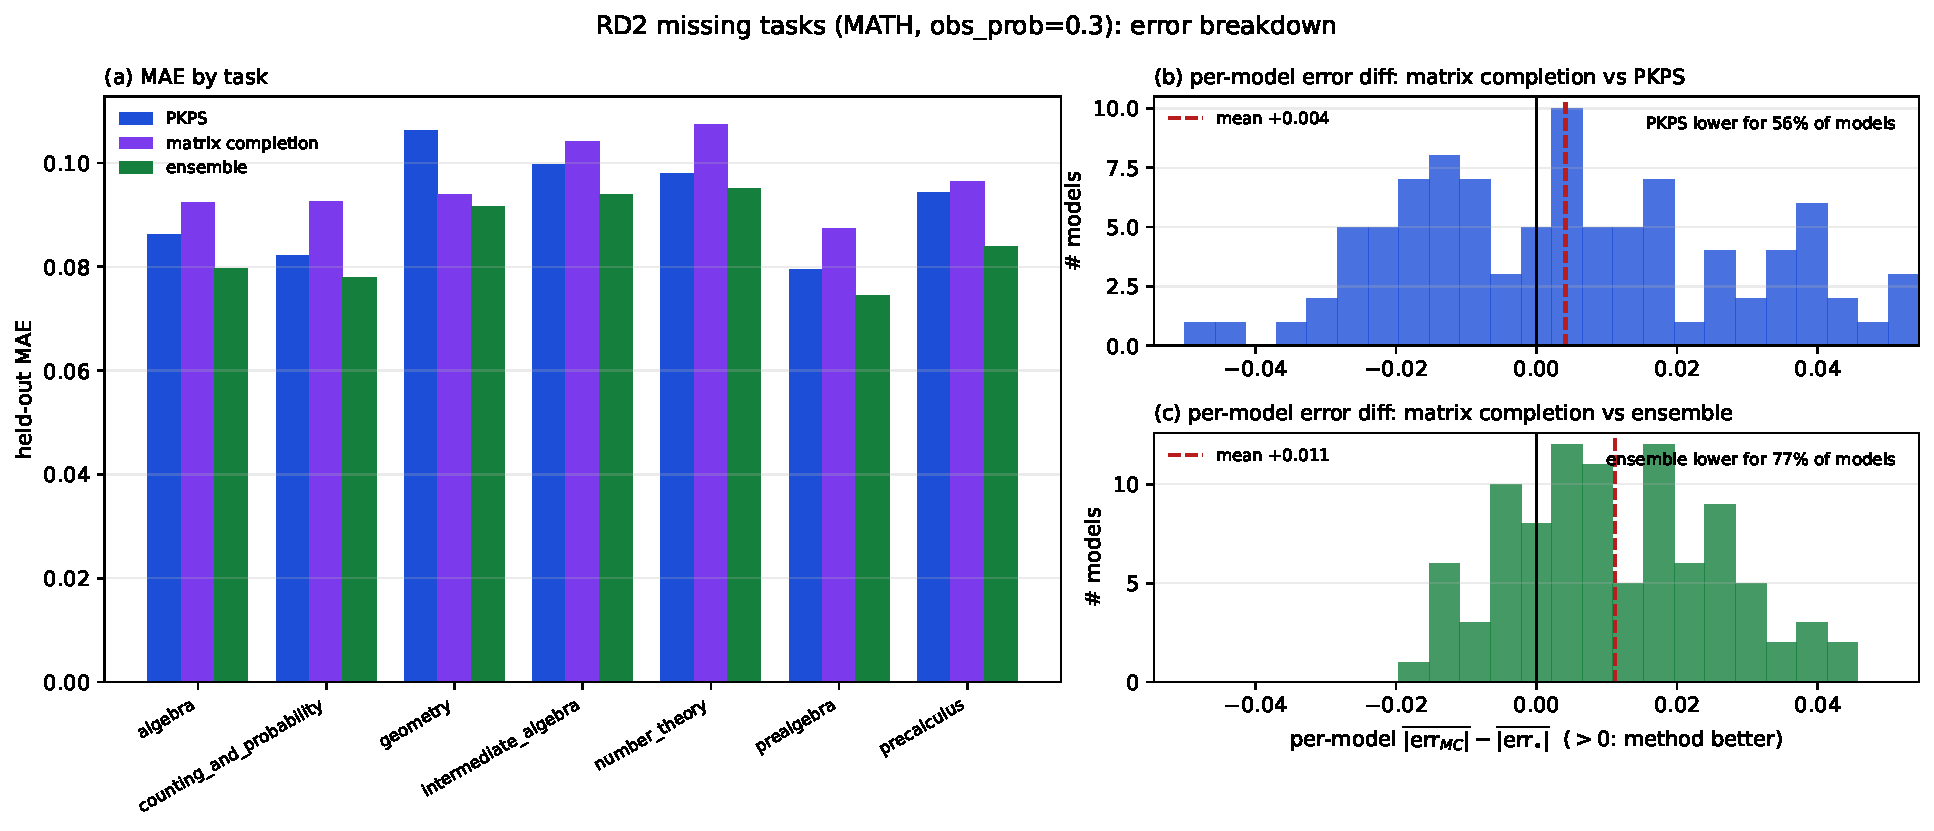
\includegraphics[width=\textwidth]{fig_rd2_breakdown.pdf}
\caption{Error breakdown (MATH, obs.\ prob.\ $0.3$). (a) The ensemble has the lowest
MAE on all seven subjects. (b,c) It shifts the whole per-model error distribution
down relative to matrix completion (lower for $77\%$ of models), so the gain is
broad rather than driven by a few models.}
\label{fig:rd2breakdown}
\end{figure}

\section{A joint heterogeneous suite}
\label{sec:joint}
The single-dataset studies use MATH as a running example to build intuition. Our main
result puts both regimes on one realistic, organically-assembled benchmark: a suite
of $18$ tasks across four datasets with very different response types---\textbf{MATH}
($7$ math-reasoning subjects), \textbf{WMT-14} ($5$ translation directions),
\textbf{MedQA} (medical multiple-choice), and \textbf{LegalBench} ($5$ legal
classification subsets)---restricted to the $93$ models evaluated on all four.

\paragraph{A block-diagonal product kernel.} MATH and WMT produce rich free-text
responses (worked solutions, translations) whose Gemini embeddings carry signal, but
MedQA and LegalBench responses are single tokens (a choice letter, a class label) for
which text embeddings are degenerate. We therefore represent each dataset's responses
natively---Gemini embeddings for the free-text datasets, one-hot answer encodings for
the single-token ones (so a linear $k_R$ measures answer agreement)---and place them
in \emph{disjoint blocks} of the response space. With a linear response kernel this
makes $k_R$ exactly zero across datasets, while a single shared query embedding with a
\emph{within-domain} bandwidth keeps $k_Q$ near zero across domains: the product
kernel automatically factorizes by domain, bridging similar queries within a dataset
and never forcing a spurious comparison between a proof and a legal label. The rest of
the pipeline is unchanged.

\paragraph{Efficient evaluation (missing queries).} Each model answers only $m$
queries per task; we estimate every (model, task) full score
(Figure~\ref{fig:rd1suite}). Because all tasks are observed---only queries are
missing---matrix completion does not apply, and this is \PKPS's regime. The
\PKPS\,$+$\,sample ensemble dominates naive sampling at every budget and on all four
datasets, roughly \emph{halving} the error at small budgets (suite-wide MAE $0.13$
vs.\ $0.29$ at one query per task; $0.093$ vs.\ $0.135$ at four). \PKPS alone is weaker
because the cross-model perspective discards a model's own answered queries; the
ensemble combines the two. IRT, the standard efficient-benchmarking baseline, needs a
dense paired block per task and is off-scale in this sparse, heterogeneous regime.

\begin{figure}[t]
\centering
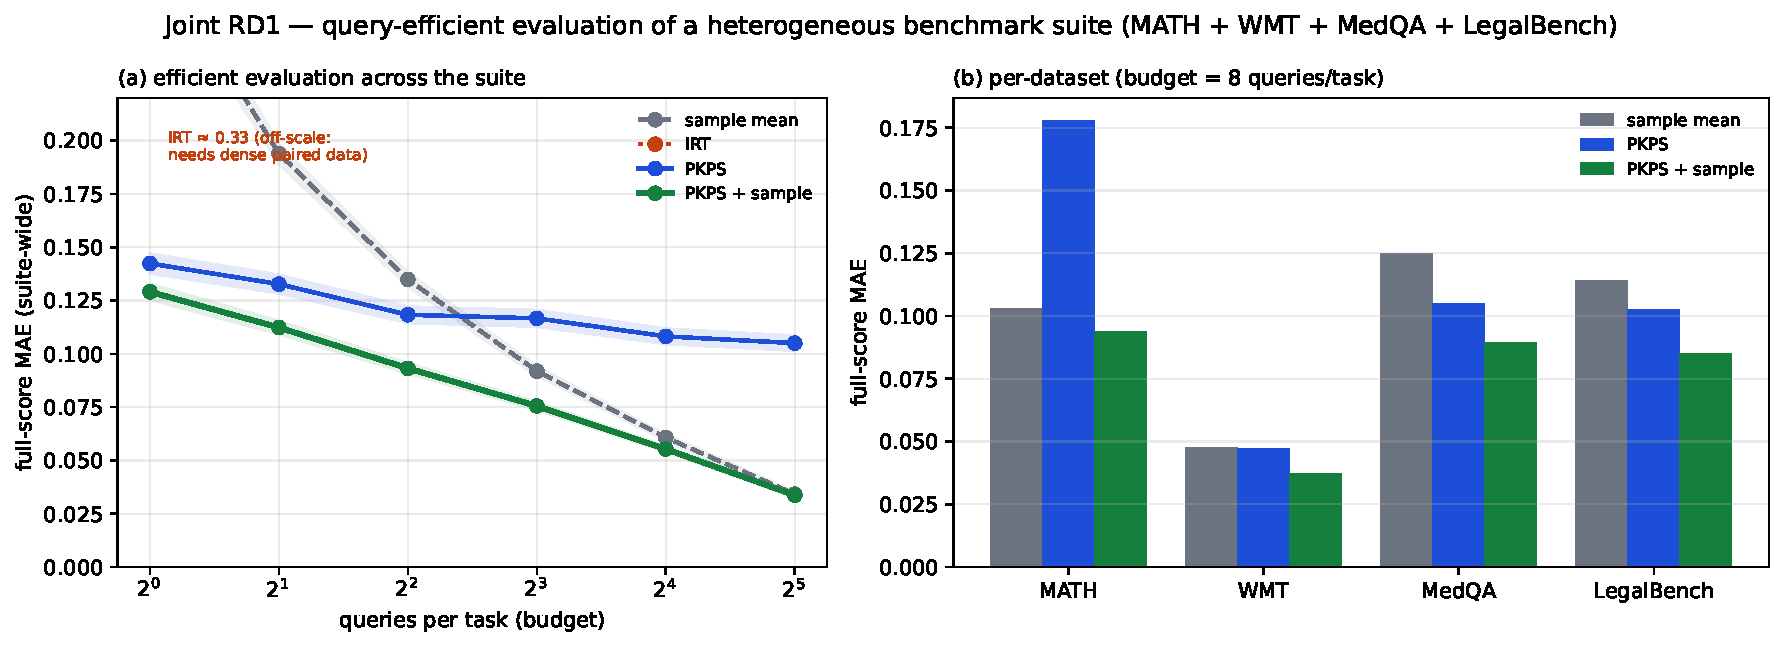
\includegraphics[width=\textwidth]{fig_rd1_suite.pdf}
\caption{Joint efficient evaluation across the suite (full-score MAE). (a) The
\PKPS\,$+$\,sample ensemble dominates naive sampling at every query budget; IRT is
off-scale. (b) The ensemble is lowest on all four datasets at four queries per task.}
\label{fig:rd1suite}
\end{figure}

\paragraph{Benchmark completion (missing tasks).} Predicting held-out (model, task)
cells of the joint matrix is, by contrast, matrix completion's regime: capable models
tend to be capable across all four domains, so the $18$-task matrix is dominated by a
single general-ability factor and is highly low-rank. \PKPS's response perspective,
which excels at separating closely-related MATH subjects, has little to add once the
target is a model's deviation from its general ability---exactly what the low-rank
model already captures (we confirmed this is intrinsic, not an artifact of the joint
embedding, across several perspective variants). Matrix completion is therefore the
stronger single method here; the \PKPS ensemble tracks it and remains the most robust
choice, never losing by more than the noise and recovering its margin when models are
scarce (Figure~\ref{fig:rd2suite}). Together the two regimes delineate where the
response perspective helps: it is decisive for query efficiency and for low-rank-poor,
heterogeneous-within-domain completion (MATH), and reduces to the low-rank view as the
benchmark matrix becomes rank-one (WMT, the joint suite).

\begin{figure}[t]
\centering
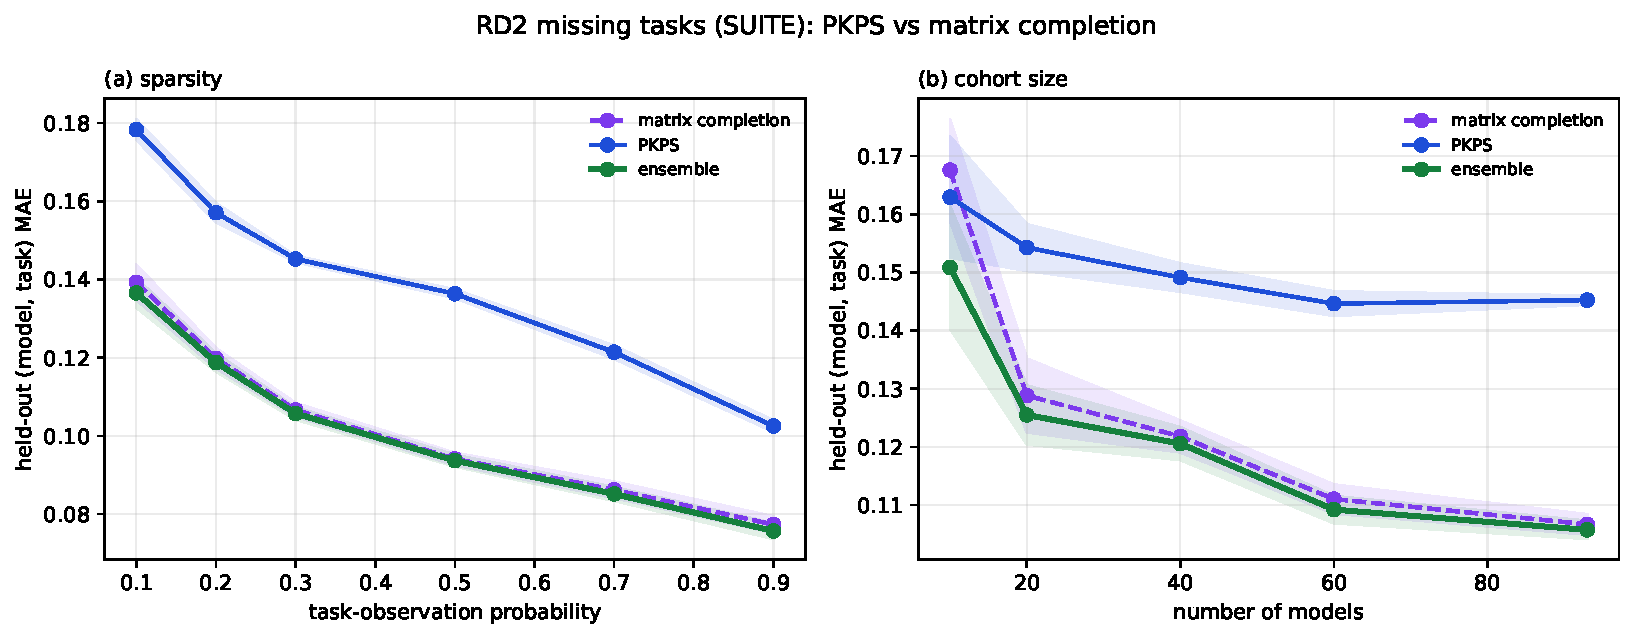
\includegraphics[width=\textwidth]{fig_rd2_suite.pdf}
\caption{Joint benchmark completion (held-out MAE). The $18$-task matrix is low-rank,
so matrix completion is strong and \PKPS trails; the ensemble (green) tracks matrix
completion and is the most robust predictor across sparsity (left) and cohort size
(right).}
\label{fig:rd2suite}
\end{figure}

\section{Related work}
\textbf{Efficient benchmarking} reduces evaluation cost by scoring on a subset of
items: item-response theory \citep{polo2024tinybenchmarks, rasch1960} and anchor
points \citep{vivek2024anchor} select informative items, while DKPS
\citep{dkps_qeff} predicts from cached responses in a perspective space. These assume
a paired/anchored design. \textbf{Benchmark completion} treats the score matrix as
low-rank and imputes missing entries \citep{benchpress, mazumder2010softimpute}; this
uses only scores, not responses. \PKPS unifies the two settings through a single
product-kernel mechanism that consumes unpaired responses, and we show it is
complementary to the score-only low-rank view.

\section{Conclusion}
\PKPS extends data-kernel perspective spaces to the sparse, unpaired evaluations that
real benchmarks produce, with classical DKPS as its $\sigma\!\to\!0$ limit and a
cheap, cross-validated bandwidth. On a single heterogeneous suite of $18$ tasks and
$93$ models---math, translation, medical QA, and legal classification---a
block-diagonal product kernel handles rich-text and single-token responses together
and roughly halves the cost of query-efficient evaluation. Our experiments also map
\emph{where} the response perspective helps: it is decisive for efficient
benchmarking and for completing heterogeneous, low-rank-poor matrices (MATH), and
reduces gracefully to the low-rank view as the benchmark matrix approaches rank one
(WMT, the joint suite). Across every regime the \PKPS--baseline ensemble is the most
robust predictor, since the response-embedding and score-only signals are
complementary. This makes score prediction practical for organically-assembled
leaderboards, where pairing cannot be assumed.

\bibliographystyle{plainnat}
\bibliography{references}
\end{document}
